% ICASSP 2027 submission -- draft.
% spconf.sty and IEEEbib.bst in this directory come from the official
% ICASSP 2027 kit (ICASSP2027_Paper_Templates/). Both are byte-identical to the
% 2026 kit's, so no layout changed when the 2027 kit replaced it.
% Deadline: 16 September 2026. Limit: 5 pages, of which the 5th may hold only
% references, funding acknowledgements and the ethics statement.
\documentclass{article}
\usepackage{spconf,amsmath,amssymb,graphicx,booktabs,microtype,xcolor,hyperref}
% Table 1 highlights: blue where the relation lands, red where it does not
\definecolor{hi}{HTML}{1F62B8}
\definecolor{lo}{HTML}{C0392B}
\renewcommand{\topfraction}{0.92}
\renewcommand{\bottomfraction}{0.6}
\renewcommand{\textfraction}{0.08}
\renewcommand{\floatpagefraction}{0.75}
\setcounter{topnumber}{3}
\setcounter{bottomnumber}{2}
\setcounter{totalnumber}{4}

\title{What Hides Musical Geometry in Audio Representations?}

% Superscript affiliations rather than \twoauthors: the first author holds
% both, and side-by-side address blocks cannot show a shared one.
\name{Junyoung Koh$^{1,2}$, Hao-Wen Dong$^{2}$
      \thanks{Code, pre-registrations and all run artifacts:
\url{https://github.com/Junst/topo-music}.}}
\address{$^{1}$Yonsei University, Seoul, Republic of Korea\\
  $^{2}$University of Michigan, Ann Arbor, MI, USA}
\begin{document}
\ninept
\maketitle

\begin{abstract}
Learned representations are often evaluated by how well their attributes can be decoded, but decodability does not imply that a representation's ambient geometry reflects the relations among those attributes. Music makes the distinction testable, since relations between keys and between pitches are explicitly defined. Across nine audio representations, linear decoding, class-centroid geometry and readout geometry dissociate: a log-frequency spectrogram matches a self-supervised encoder at decoding key while showing no circle-of-fifths structure among its centroids, though its probe weights carry that structure strongly. Two factors govern how visible the geometry is: the number of examples behind each class centroid, which moves fifths geometry 13.4-fold where a thousandfold change in pooling duration moves it 1.7-fold, and the metric, under which octave equivalence absent from ambient distances is recovered by a rank-4 projection fitted on key labels alone. Helical pitch organization dissociates from octave equivalence in turn, the best helix fit belonging to the representation with no octave contrast.
\end{abstract}

\begin{keywords}
music representation learning, probing, representation geometry, key detection,
octave equivalence
\end{keywords}

\section{Introduction}
\label{sec:intro}

Self-supervised music audio encoders support linear probes
\cite{probes} for key, pitch, genre, and instrument \cite{mert,marble}, and probe performance is commonly used to assess what information their representations make accessible. Yet successful
decoding establishes accessibility, not the geometric form in which that
information is organized. Two representations can support similarly accurate linear classifiers while arranging the corresponding classes differently in their embedding spaces. Music provides a direct setting for separating these questions because its attributes come with explicit relational structure. Musical keys are not merely 24 category labels: their relationships are organized by structures such as the circle of fifths and Krumhansl--Kessler profiles. Likewise, pitch contains both pitch height and pitch class, with octave equivalence relating notes separated by twelve semitones. These structures make it possible to ask not only whether key or pitch can be decoded, but whether distances within a representation reflect the expected relations between them.

We examine the same musical classes using three measurements, summarized in Table~\ref{tab:measures}. Linear decoding measures how well class information can be recovered by a linear probe. We use class-centroid geometry to refer to the distances among class means in the
original representation space, and probe-weight geometry to the distances among the
corresponding classifier weights. Both are read by correlating those distances with
a reference structure, as in representational similarity analysis \cite{rsa}.

Across nine audio representations, these measurements reveal distinct geometric profiles. We identify two factors that determine when musical geometry becomes visible. At the audio-clip level, circle-of-fifths geometry depends much more strongly on the number of examples used to estimate each key centroid than on temporal pooling duration. At the note level, octave equivalence depends strongly on the metric. Structure absent from ambient distances can remain weakly visible on a local manifold or become pronounced under a low-rank projection learned solely from key labels. We further show that helical pitch organization dissociates from octave equivalence, demonstrating that different geometric measurements of the same musical relation need not agree.

\begin{table}[t]
\centering
\footnotesize
\setlength{\tabcolsep}{4pt}
\caption{The three measurements, all computed on the same clips, the same 24 keys and the same probe.}
\label{tab:measures}
\begin{tabular}{@{}l p{0.85\columnwidth}@{}}
\toprule
F1 & \textbf{How easily key can be read out.} Macro-F1 of a multinomial
logistic probe over 24 keys, folds grouped by track. \\
\addlinespace[2pt]
$\rho^{\text{cent}}_{5}$ & \textbf{Whether the representation space is itself
arranged by key relation.} Spearman correlation between the pairwise distances
of the 24 key centroids and circle-of-fifths distance. \\
\addlinespace[2pt]
$\rho^{W}_{5}$ & \textbf{Whether the directions the probe learns are arranged
the same way.} The same correlation on the pairwise distances of its 24 class
weight vectors. \\
\bottomrule
\end{tabular}
\end{table}

\begin{table*}[t]
\centering
\small
\caption{Key information, ambient geometry and readout geometry come apart. All columns are measured on the same 7035 GiantSteps clips and the same 24 keys. \textit{acc}: 24-way key accuracy from the pooled clip embedding (chance $.042$). $\rho^{\text{cent}}_{5}$: circle-of-fifths correlation among the 24 key centroids, i.e.\ the ambient metric; $\rho_{5}\!\mid\!\text{spec}$ partials out mel-spectral centroid distance. $\rho^{W}_{5}$: the same correlation among the fitted probe's 24 class weight vectors, i.e.\ what a linear readout can reach. $\rho_{\text{chr}}$ (semitone adjacency) and $\rho_{\text{mode}}$ (major/minor) are reported as discriminants. The control block fixes the scale: an analytic circle of fifths scores $\approx\!1$ everywhere; random features carry no information and show nothing; orthogonal per-key codes decode key better than any real representation ($.651$) with equidistant classes by construction, and show nothing either -- so $\rho^{W}_{5}$ is not an artefact of an accurate classifier on this label set.}
\label{tab:decodable-vs-geometric}
\begin{tabular}{l r r r r r r r}
\toprule
representation & acc & $\rho^{\text{cent}}_{5}$ & $\rho_{5}\!\mid\!\text{spec}$ & $\rho^{W}_{5}$ & $z_W$ & $\rho_{\text{chr}}$ & $\rho_{\text{mode}}$ \\
\midrule
\multicolumn{8}{l}{\textit{Controls}} \\
\quad analytic fifths (metric ctrl) & $0.274$ & $+0.977$ & $+0.977$ & $+0.986$ & $+15.8$ & $-0.085$ & $+0.053$ \\
\quad random features (no info) & $0.055$ & $+0.009$ & -- & $+0.033$ & $+0.6$ & $-0.001$ & -- \\
\quad orthogonal key codes (no tonal rel.) & $0.651$ & $-0.008$ & -- & $-0.005$ & $-0.1$ & $-0.001$ & -- \\
\multicolumn{8}{l}{\textit{Spectral front end (fold $\times$ norm)}} \\
\quad log-CQT, 84 bin, dB & $0.492$ & $-0.035$ & $-0.103$ & $+0.560$ & $+9.1$ & $+0.174$ & $+0.165$ \\
\quad log-CQT, 84 bin, per-frame norm & $0.486$ & $-0.117$ & $-0.136$ & $+0.671$ & $+10.6$ & $+0.491$ & $+0.013$ \\
\quad octave-summed, 12 bin, dB & $0.407$ & $-0.106$ & $-0.157$ & $+0.305$ & $+4.9$ & $+0.391$ & $-0.088$ \\
\quad chromagram (fold + norm) & $0.451$ & $+0.475$ & $+0.445$ & $+0.692$ & $+11.0$ & $+0.140$ & $-0.054$ \\
\multicolumn{8}{l}{\textit{Neural codec}} \\
\quad EnCodec 32 kHz & $0.404$ & $+0.177$ & $+0.218$ & $+0.648$ & $+10.4$ & $+0.041$ & $+0.098$ \\
\multicolumn{8}{l}{\textit{MERT-v1-330M}} \\
\quad layer 4 & $0.451$ & $+0.445$ & $+0.432$ & $+0.412$ & $+6.8$ & $-0.025$ & $+0.216$ \\
\quad layer 12 & $0.456$ & $+0.468$ & $+0.455$ & $+0.428$ & $+7.1$ & $+0.024$ & $+0.203$ \\
\quad layer 16 & $0.440$ & $+0.395$ & $+0.377$ & $+0.409$ & $+6.8$ & $+0.047$ & $+0.262$ \\
\quad layer 24 & $0.418$ & $+0.294$ & $+0.266$ & $+0.484$ & $+7.6$ & $+0.049$ & $+0.328$ \\
\bottomrule
\end{tabular}
\end{table*}


\begin{figure}[tb]
\centering
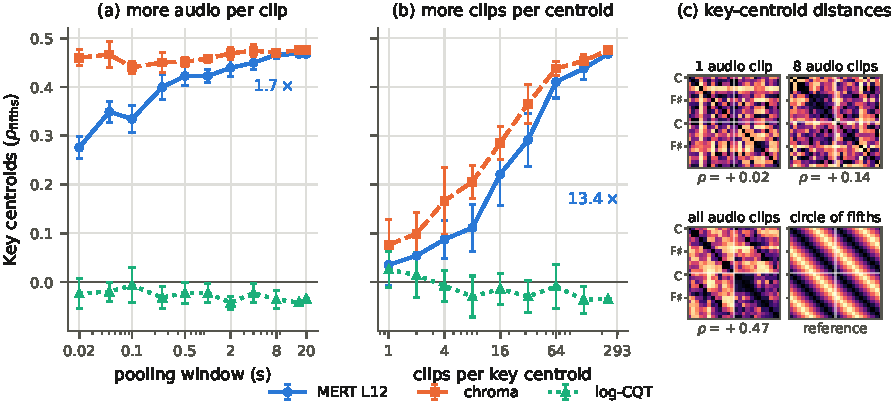
\includegraphics[width=\columnwidth]{figs/fig1_averaging.pdf}
\caption{Clip-level fifths geometry depends far more on the number of audio clips per centroid (b) than on temporal context (a). Error bars are one standard deviation over 5 and 10 draws.}
\label{fig:averaging}
\end{figure}

\section{Related Work}
\label{sec:related}

\noindent\textbf{Probing Audio Representations.}
Linear probes are the standard instrument for asking what a representation
encodes \cite{probes}, and music audio encoders are routinely evaluated this way, with MERT \cite{mert} and MARBLE \cite{marble} reporting probe accuracy for key, pitch, genre and instrument. Castellon et al. \cite{castellon2021} similarly evaluate music representations through shallow probes, including key detection. Hewitt and Liang \cite{controltasks} argue that probe performance should be
interpreted relative to control tasks designed to measure probe selectivity,
Voita and Titov \cite{voita2020} recast the measurement as description length
rather than accuracy, and Belinkov \cite{belinkov2022} surveys what the
instrument can and cannot support. A parallel line compares two representations
to each other, as in centered kernel alignment \cite{cka}, whereas we ask
whether one representation matches a relational structure specified in
advance.

\noindent\textbf{Tonal Geometry.}
Music cognition has established well-defined relational structures for both key and pitch. Perceived key relationships follow the circle of fifths and Krumhansl--Kessler profiles \cite{krumhansl1982,krumhansl1990}, while pitch perception separates pitch height from chroma \cite{shepard1982}. Chroma features \cite{brown1991,librosa} encode octave equivalence by construction and therefore provide a positive control for these relationships. Tonality-aware objectives such as STONE \cite{stone} explicitly impose key
equivariance during training. Pilataki et al. \cite{pilataki2025} report a related observation in a JEPA-based transcription model, where NSynth embeddings show strong separation by timbre and pitch height but weak separation by pitch class. Closest to the octave measurements, Yagi et al. \cite{yagi2026} fit a parametric helix to principal components of
Jukebox \cite{jukebox} and MusicGen \cite{musicgen} representations of
synthesized isolated notes, and report a helical arrangement whose clarity varies with the instrument and with the harmonic content of the signal.

\section{Method}
\label{sec:method}

\begin{figure}[tb]
\centering
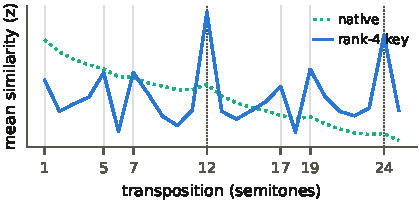
\includegraphics[width=\columnwidth]{figs/fig2_curve.pdf}
\caption{A rank-4 projection fitted only on GiantSteps track tonics and applied unchanged to NSynth. The projected curve peaks at exactly twelve and twenty-four semitones, where
the native one only falls off with distance.}
\label{fig:mechanisms}
\end{figure}

\noindent\textbf{Representation decomposition.} We decompose the representation $z$ of a sample with class label $y$ as
\begin{equation}
z = s_y + n_y + \varepsilon, \qquad \mathbb{E}[\varepsilon \mid y] = 0,
\label{eq:decomp}
\end{equation}
\noindent where $s_y$ is the class-dependent signal whose relations encode the structure of interest, $n_y$ is other class-dependent variation and $\varepsilon$ is the residual. Averaging examples from the same class reduces $\varepsilon$ but not $n_y$, whereas a change of metric can alter how $s_y$ and $n_y$ contribute to the measured geometry.

\noindent\textbf{Representations.} We consider three self-supervised music encoders,
MERT-v1-330M \cite{mert}, MuQ-large \cite{muq} and MATPAC++ \cite{matpac}, evaluated at matched relative depths. MuQ and MATPAC++ have half as many layers as MERT. We also include PupuJEPA \cite{pupujepa}, a music-domain JEPA over mel patches, using its teacher encoder, and EnCodec 32\,kHz \cite{encodec}, a neural codec used by MusicGen  \cite{musicgen}. The log-frequency representations comprise a log-CQT \cite{brown1991,librosa} at 12 bins per octave, an HCQT \cite{hcqt} at 60 bins per octave stacked over six harmonics, and a multi-scale pitch-quantized STFT at 60 bins per octave. A CQT chromagram \cite{librosa} folds octaves into 12 pitch classes and serves as a positive control. Frame-level representations are averaged over time to obtain one vector per clip.

\noindent\textbf{Datasets.} GiantSteps \cite{giantsteps} contains 7,035 clips covering all 24 keys from 1,763 tracks, all within electronic dance music. FMAK \cite{fmak} contains 5,476 usable tracks with expert key and mode annotations across 17 genres. We use one excerpt per track, preventing overlap across splits and reducing genre-specific confounding of key.

\noindent\textbf{Key and readout geometry.} In addition to the circle of fifths, centroid distances are compared with Krumhansl–Kessler key-profile distance and semitone distance ($\rho_{\text{chr}}$). The fifths and semitone references are nearly uncorrelated ($\rho=-0.038$). Significance is assessed with 2,000 permutations of the key labels. Partial Spearman correlation additionally controls for mel-spectral centroid distance. Probe folds are grouped by track.

\noindent\textbf{Octave equivalence.} On NSynth \cite{nsynth}, we use only real recordings and exclude signal-processed pitch shifts. For each instrument, a fixed anchor set supports all transpositions up to 25 semitones. We measure the mean cosine similarity between each note and its transposition by k semitones. We report three preregistered statistics. The local contrast compares 12 semitones with the mean of 11 and 13 semitones, the strict contrast compares it with the maximum similarity from 8 to 11 semitones, and the periodic coefficient is obtained from a fitted twelve-semitone periodic term. Confidence intervals are bootstrapped over instruments, and all three statistics are required to agree in sign.

\noindent\textbf{Metrics.} We compute the octave statistics under three metrics on the same recordings. The native metric uses cosine distance in the original representation space. The geodesic metric uses shortest-path distance on a
symmetric $k$-nearest-neighbor graph with cosine-weighted edges, as in Isomap
\cite{isomap}. We sweep k from 5 to 50 and report unreachable pairs without imputation. The supervised metric is induced by the linear projection described below. Distances are negated before computing the contrasts, so positive values consistently indicate stronger octave equivalence.

\noindent\textbf{Subspaces.} We construct each supervised subspace from the top $d$
Ledoit--Wolf shrinkage-LDA \cite{ledoit2004} discriminant directions for the specified target, with $d\leq11$, the maximum rank for a twelve-class target. We report the fraction of total variance retained by each subspace. Matched random orthonormal subspaces control for the
effect of dimensionality reduction itself. As a supervised null we repeat the
same fit after permuting the GiantSteps key labels across tracks, which leaves
the label distribution and the several-clips-per-track structure intact and
destroys only the correspondence with audio, and report the resulting NSynth
contrast over 200 draws.

\noindent\textbf{Helical organization.} We also fit the parametric pitch helix
of Yagi et al.~\cite{yagi2026}, which measures a different property of the same
notes. For each instrument we average every pitch over a contiguous
three-octave window, the span they use, and keep the 66 evaluation instruments
that cover one. We apply PCA to those pitch means, enumerate the ten
three-component projections of the top five components, fit the nine-parameter
helix to each, and report the best. Their score is an inverse mean squared
error and therefore depends on the scale of the embedding, so we report the
fraction of pitch-centroid variance the helix explains, and read it against the
same fit after the pitch order is shuffled, which leaves the point cloud intact
and destroys only its correspondence with pitch.


\begin{table}[t]
\centering
\footnotesize
\setlength{\tabcolsep}{1.5pt}
\caption{Centroid geometry, readout geometry and the chromatic control, measured on FMAK rather than GiantSteps: 5476 tracks over 17 genres, one excerpt per track. The three $\Delta$ columns are the NSynth octave contrast under the native metric and after a rank-4 projection fitted on GiantSteps and on FMAK keys. $\Delta^{\mathrm{nat}}$ is measured on NSynth alone and so does not depend on the corpus.}
\label{tab:fmak}
\resizebox{\columnwidth}{!}{%
\begin{tabular}{l r r r r r r}
\toprule
representation & $\rho^{\text{cent}}_{5}$ & $\rho^{W}_{5}$ & $\rho_{\text{chr}}$ & $\Delta^{\mathrm{nat}}$ & $\Delta^{\mathrm{GS}}$ & $\Delta^{\mathrm{FM}}$ \\
\midrule
\multicolumn{7}{l}{\textit{Spectral representations}} \\
\hspace{3pt}log-CQT~\cite{brown1991} & $+0.057$ & $+0.474$ & \textcolor{hi}{$\mathbf{-0.046}$} & $+0.004$ & $+0.466$ & $+0.507$ \\
\hspace{3pt}HCQT~\cite{hcqt} & $+0.389$ & $+0.167$ & \textcolor{lo}{$\mathbf{-0.092}$} & $+0.011$ & $+0.535$ & $+0.421$ \\
\hspace{3pt}PQ-STFT & $+0.454$ & $+0.263$ & $-0.055$ & \textcolor{hi}{$\mathbf{+0.227}$} & \textcolor{hi}{$\mathbf{+0.603}$} & \textcolor{hi}{$\mathbf{+0.513}$} \\
\hspace{3pt}chromagram~\cite{librosa} & $+0.632$ & $+0.496$ & $-0.092$ & $+0.698$ & $+0.878$ & $+0.689$ \\
\multicolumn{7}{l}{\textit{Neural codec}} \\
\hspace{3pt}EnCodec~\cite{encodec} & $+0.207$ & $+0.421$ & $-0.076$ & $+0.000$ & $+0.459$ & $-0.001$ \\
\multicolumn{7}{l}{\textit{Learned encoders}} \\
\hspace{3pt}MERT L12~\cite{mert} & $+0.437$ & $+0.102$ & $-0.068$ & $-0.003$ & $+0.223$ & $+0.197$ \\
\hspace{3pt}MuQ L6~\cite{muq} & $+0.467$ & $+0.184$ & $-0.068$ & $+0.034$ & $+0.307$ & $+0.204$ \\
\hspace{3pt}MATPAC L6~\cite{matpac} & \textcolor{hi}{$\mathbf{+0.597}$} & \textcolor{lo}{$\mathbf{-0.064}$} & $-0.091$ & $+0.010$ & $+0.114$ & $+0.069$ \\
\hspace{3pt}PupuJEPA~\cite{pupujepa} & \textcolor{lo}{$\mathbf{+0.031}$} & \textcolor{hi}{$\mathbf{+0.489}$} & $-0.078$ & \textcolor{lo}{$\mathbf{-0.004}$} & \textcolor{lo}{$\mathbf{+0.006}$} & \textcolor{lo}{$\mathbf{-0.002}$} \\
\bottomrule
\end{tabular}}
\end{table}



\section{Results}
\label{sec:results}

\subsection{Information, metric and readout dissociate}

\label{sec:three}
The controls in Table~\ref{tab:decodable-vs-geometric} establish that decodability alone does not imply fifths geometry. Orthogonal per-key codes achieve higher key F1 than any real representation while showing no fifths structure in either centroid or probe-weight geometry.

The log-CQT provides a direct example of this dissociation. It outperforms MERT layer 12 in grouped key decoding while showing no fifths structure in its centroids, despite strong fifths structure in its probe weights ($\rho^W_5=0.560$). Randomly shuffled folds inflate performance for several representations and
reverse the log-CQT--MERT comparison, motivating track-grouped evaluation
throughout. The inflation is far from uniform, adding 0.33 to MERT layer 12 and
to the pitch-quantized STFT but 0.03 to the chromagram, so the leak is largest
where a representation can identify the track rather than the key.

Across depth, centroid and probe-weight geometry move in opposite directions in all three learned music encoders, while key F1 does not systematically improve. To control for post-hoc layer selection, we also follow MARBLE and learn a softmax-weighted combination of all hidden layers jointly with the probe. The weighted models match or slightly underperform the swept best layers when both are fitted with the same optimizer, with learned weights concentrating near the selected layers for MuQ and MATPAC.

The centroid--readout dissociations persist on FMAK, with no representation reversing its relative pattern. Chromatic proximity differs across corpora, appearing for several spectral representations on GiantSteps but not on FMAK.


\subsection{Sample-limited masking}
\label{sec:sample}

Fig.~\ref{fig:averaging}(a) shows relatively limited changes with pooling duration for most representations, with EnCodec as the main exception.
By contrast, increasing the number of clips per centroid produces a much larger change. MERT L12 rises from 0.035 to 0.468, a 13.4-fold increase compared with 1.7-fold across the thousandfold pooling-duration sweep. With one example per centroid, fifths geometry is indistinguishable from zero for every representation.

This pattern is consistent with a dominant contribution from $\varepsilon$ in Eq.~\eqref{eq:decomp}, as within-key variation across tracks is reduced when more examples contribute to each centroid.

\subsection{Octave equivalence depends on the metric}
\label{pg:s43}
\label{sec:metric}

Under the native metric and the sign-consistency criterion registered in
advance, MuQ shows a weak but reliable effect at every layer, whereas MERT and
the codec largely fail it. Averaging NSynth recordings into pitch centroids recovers no reliable effect
in MERT, so the near-zero geometry is not finite-sample variation alone. A $k$-nearest-neighbor geodesic metric reveals small but reliable effects in
MERT layers 4 and 12 and in EnCodec, stable for $k$ from 5 to 50, but not in
layer 24. MERT layer 12 changes from $-0.003$ under the native metric to 0.012 under the
geodesic one. Octave structure can therefore be absent from global distances, weakly
preserved on the manifold, or visible only after supervised reweighting, and
the geodesic metric is not uniformly more revealing.

The $\Delta^{\mathrm{nat}}$ column of Table~\ref{tab:fmak} shows that this
metric dependence is not specific to learned representations, only the
pitch-quantized STFT carrying substantial native octave structure.

\noindent\textbf{Transfer of the supervised projection.} The projection is
fitted only to GiantSteps tonic labels, with no notes and no octave
information, and applied unchanged to NSynth recordings. It raises the strict
contrast to 0.346 for MuQ layer 2, and Fig.~\ref{fig:mechanisms} shows the curve, with maxima at exactly twelve and twenty-four semitones. Refitting it on
FMAK keys and applying it unchanged to the same recordings reproduces the
transfer for MERT and the log-CQT, at 0.197 for MERT layer 12 against 0.223
from GiantSteps, even though MERT's clip-level readout geometry falls from
0.428 to 0.102 between the corpora, so the transfer does not depend on the corpus the projection was fitted on.

\noindent\textbf{Alternative projections and nulls.}
Fig.~\ref{fig:subspaces} compares rank-4 subspaces fitted to different targets. Pitch-class supervision recovers octave equivalence for several representations, whereas pitch-height supervision does not show the same pattern. Permuting the key labels across tracks reduces the contrast to near the unfitted level, with none of 200 permutations reaching the true-label result for any learned encoder. The key-supervised effect therefore depends on the correspondence between audio and key labels rather than on supervised low-rank projection alone. The permuted-label contrast is higher for the chromagram and pitch-quantized STFT, reaching 0.18 and 0.21, respectively, but remains below 0.04 for the learned encoders. The effect is also stable across projection rank for MERT layer 12, emerging at $d=2$ and remaining between 0.21 and 0.24 through $d=11$. PupuJEPA provides a contrasting case: its key-supervised contrast is near zero, while pitch-class supervision reaches 0.174, indicating that the null key-transfer result does not imply an absence of octave structure under other metrics. The learned subspaces retain less than 0.3\% of the variance in NSynth.

\noindent\textbf{Helical organization.}
Helicality measures a different geometric property from the preceding octave contrasts. A helix separates octaves along its height axis rather than identifying them. On the same notes, helical fit and octave equivalence rank the representations oppositely: MERT layer 12 has the strongest helix fit but weak octave equivalence, whereas the chromagram shows the reverse (Fig.~\ref{fig:helix}).

Key supervision does not guarantee pitch-height invariance, since GiantSteps key labels may correlate with subgenre, tempo or production, though the transfer rules out an explanation resting only on GiantSteps-specific nuisance correlations. Nor is it mechanistic: whether the projection suppresses or amplifies is not identifiable here.

\noindent\textbf{A failed registered prediction.} We predicted that removing the recovered subspace, in the manner of nullspace
projection \cite{inlp} and amnesic probing \cite{amnesic}, would at least
halve clip-level fifths geometry. Against a baseline recomputed on the same held-out
clips it barely moves, from 0.127 to 0.119 for MERT layer 12, and only the
twelve-dimensional chromagram collapses.
The subspace is therefore sufficient to expose the relation without
exclusively containing it.

\begin{figure}[tb]
\centering
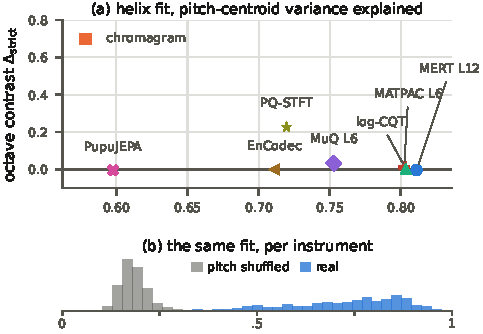
\includegraphics[width=\columnwidth]{figs/fig4_helix.pdf}
\caption{Helical organization does not imply octave equivalence. (a) The two
scores order the representations in opposite directions. (b) Every
representation fits the pitch helix of Yagi et al.~\cite{yagi2026} far better
than a pitch-shuffled reference, over 528 instrument fits.}
\label{fig:helix}
\end{figure}

\begin{figure}[tb]
\centering
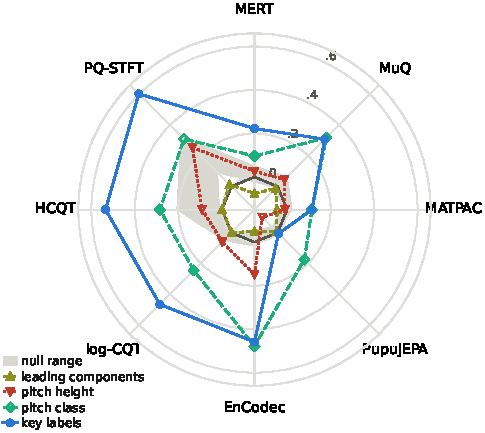
\includegraphics[width=\columnwidth]{figs/fig5_radar.pdf}
\caption{The strict octave contrast on the same NSynth notes under rank-4
subspaces differing only in their fitting target. The band spans the two nulls,
a random subspace and a permuted-label fit. Encoders are at MERT L12, MuQ L6
and MATPAC L6. The chromagram is omitted, a random rank-4 subspace of its
twelve dimensions already reaching 0.569.}
\label{fig:subspaces}
\end{figure}

\section{Discussion}
\label{pg:disc}

The results separate linear accessibility from the geometry in which musical classes are arranged. At the clip level, weak centroid geometry can result from limited class sampling, while at the note level the same musical relation changes substantially across ambient, geodesic, and supervised metrics. Probe accuracy and geometric similarity should therefore not be treated as
interchangeable evidence that a representation has learned a musical relation.
Geometric measurements depend on how examples are aggregated and how distances
are defined, and comparisons should report these choices explicitly.

\noindent\textbf{Limitations.} NSynth is monophonic, our subspaces are linear
by design, and the instrument split that separates fitting from evaluation on
NSynth is a single draw. The FMAK-fitted projection does not transfer for
EnCodec, where it falls from 0.459 to $-0.001$, so what a supervised projection
recovers from a codec latent may itself be corpus-specific. Our helix numbers
are also not directly comparable with those of Yagi et al.~\cite{yagi2026}, who
analyze different models on synthesized notes and score the fit by an inverse
mean squared error that depends on the scale of the embedding. We report the
scale-free form of the same fit and compare orderings rather than values.

\section{Conclusion}
\label{pg:concl}

We measured linear decodability, class-centroid geometry and readout geometry
for the same musical classes, across nine audio representations and three
corpora. The three come apart, and two factors account for most of the
difference: at the clip level, how many examples estimate each centroid rather
than how long each one is, and at the note level, the metric under which
distances are compared. A rank-4 subspace fitted on clip-level key labels
exposes octave periodicity in isolated notes that neither the ambient metric
nor the leading principal components reveal, and neither a permuted-label fit
nor a subspace fitted on pitch height reproduces it. Helical organization and
octave equivalence order the same representations differently, so even two
geometric readings of one relation need not agree. A musical relation therefore has no single geometric expression within a representation. Geometric claims should specify the measurement under which the structure appears.

\label{pg:endtext}

\bibliographystyle{IEEEbib}
\bibliography{refs}

\end{document}
